\documentclass{beamer}

\usepackage[utf8]{inputenc}
\usepackage[croatian]{babel}
\usepackage[T1]{fontenc}
\usepackage{listings}
\usepackage{graphicx}
\graphicspath{ {../img/} }

\usetheme{Boadilla}
\usecolortheme{whale}

\subtitle{Projekt iz bioinformatike}
\title{Računanje najduljeg zajedničkog prefiksa temeljenog na BWT}
\author[Čupić, Jurelinac, Živec]{Tonko Čupić \and Zvonimir Jurelinac \and Tomislav Živec}
\institute{Fakultet elektrotehnike i računarstva}
\date{26.01.2018.}

\begin{document}
    \frame{\titlepage}

    \begin{frame}
        \frametitle{Zadatak}
        \framesubtitle{Izgradnja polja najduljh zajedničkih prefiksa}

        \textbf{Koraci u računanju LCP polja ulaznog niza:}
        \begin{enumerate}
            \item Izračun sufiksnog polja ulaznog niza
            \item Određivanje Burrows-Wheelerove transformacije ulaza
            \item Izgradnja stabla valića nad BW-transformatom
            \item Provedba algoritama 1 i 2 (iz rada Beller et al. (2013)) koji kao rezultat daju LCP polje
        \end{enumerate}

        \vspace{1cm}

        \textbf{Sažeto:}
        $$\textit{Ulaz} \Rightarrow \textit{Sufiksno polje} \Rightarrow \textit{BWT} \Rightarrow \textit{Stablo valića} \Rightarrow \textit{LCP polje}$$

    \end{frame}

    \begin{frame}
        \frametitle{Rezultati}
        \framesubtitle{Što je sve postignuto?}

        \begin{enumerate}
            \item Parsiranje ulaza u \textbf{FASTA} formatu
            \item Izračun \textbf{sufiksnog polja} pomoću gotove \texttt{sais} biblioteke
            \item Određivanje \textbf{Burrows-Wheelerove} transformacije prema jednostavnom izrazu: $BWT[i] =S[SA[i]-1]$
            \item Izgradnja \textbf{stabla valića} (vlastita implementacija pomoću niza bitvektora)
            \item Implementacija \textbf{algoritama 1 i 2} (iz rada \textit{Beller et al. (2013)})
            \item Pohrana rezultata u datoteku
        \end{enumerate}
    \end{frame}

    \begin{frame}
        \frametitle{Rezultati}
        \framesubtitle{Ostvarene optimizacije}

        \begin{enumerate}
            \item \textbf{Uklanjanje rekurzije} (prisutna u konstrukciji stabla valića i algoritmu 1) --- zamjena s redom i stogom
            \item \textbf{Optimiziranje korištenih struktura podataka} --- obično polje umjesto hash-tablice, vlastita minimalna implementacija stoga
            \item \textbf{Brzi bitvektori} --- koncept \textit{bucketa} (kutija) -- veliki bucketi (256 bitova) za spremanje prefiksnih suma, mali (64 bita) za pohranu bitova i brzo brojenje (\texttt{popcount})
        \end{enumerate}

    \end{frame}

    \begin{frame}
        \frametitle{Rezultati}
        \framesubtitle{Konačne performanse}

        \begin{columns}[c]

        \column{.5\textwidth}
        \center \textbf{Vrijeme izvođenja}
        \begin{figure}[h!]
            \begin{center}
                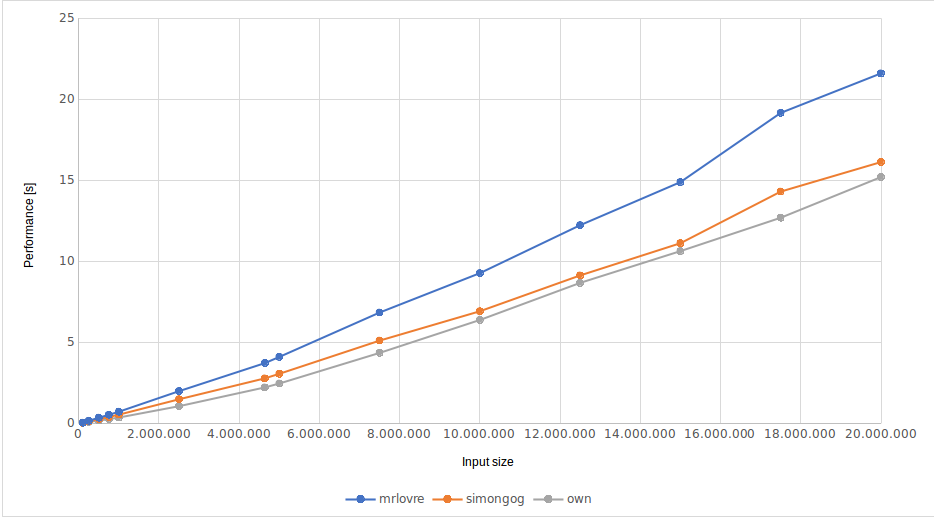
\includegraphics[width=\columnwidth]{timeGraph.png}
            \end{center}
        \end{figure}

        \column{.5\textwidth}
        \center \textbf{Zauzeće memorije}
        \begin{figure}[h!]
            \begin{center}
                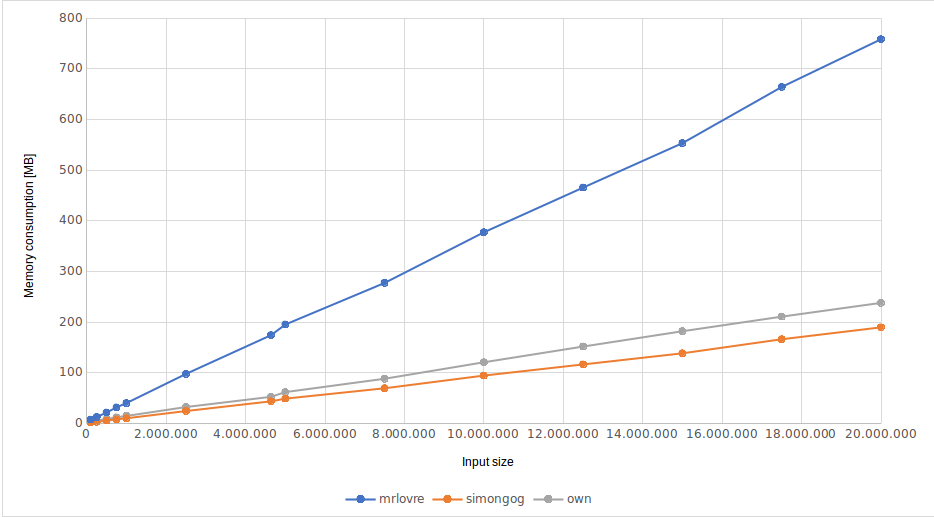
\includegraphics[width=\columnwidth]{memoryGraph.png}
            \end{center}
        \end{figure}

        \end{columns}
    \end{frame}
\end{document}
